The goal for the Supermario model is to solve a level successfully. The first level was chosen since it provides a diverse environment with different enemy types and obstacles, while not being too skill intensive to solve. 
Prior to modeling some assumptions were made to fulfill time and complexity constraints.
Only a fixed number of enemies and obstacles in the path of the player are considered in order to ensure a static input size. For this number, five has proved to be sufficient for the first level and the implemented strategy. There are rarely more than 3 enemies near the player. For the same reason only the next hole in the ground is considered.
In order to develop the model, different situations were assessed and according tests derived. Both the scenarios which a Supermario model has to master and the derived tests are listed below.

\begin{figure}[!h]
	\centering
	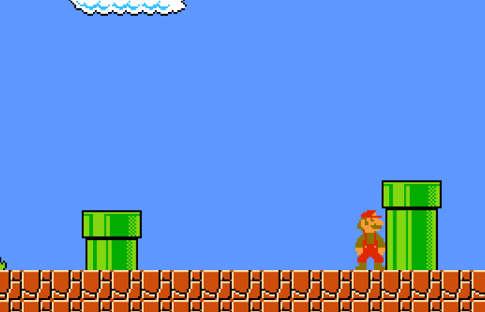
\includegraphics[scale=0.55]{pictures/Mario1.PNG}
	\caption{Mario has to go left in order jump over the obstacle}
	\label{fig:marioobstacle}
\end{figure}

\begin{figure} 
    \subfigure[Mario evades a enemy by jumping]{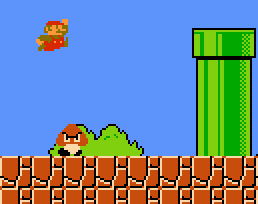
\includegraphics[width=0.49\textwidth]{pictures/haller_mario2.PNG}} 
    \subfigure[Mario defeats enemies by landing on them]{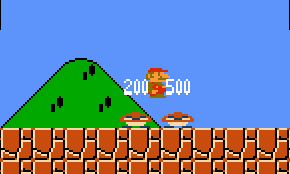
\includegraphics[width=0.49\textwidth]{pictures/haller_mario3.PNG}} 
	\caption{Mario has to jump over/to enemies} 
	\label{fig:marioenemies}
\end{figure} 

\begin{figure} 
    \subfigure[Mario and a hole in the ground]{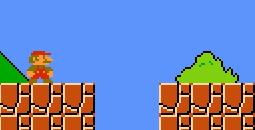
\includegraphics[width=0.49\textwidth]{pictures/haller_mario4.PNG}} 
    \subfigure[Mario and a hole with obstacles]{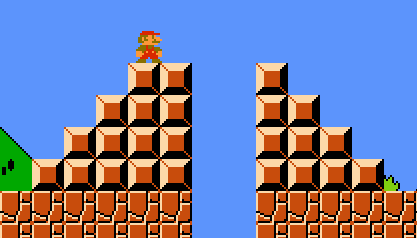
\includegraphics[width=0.49\textwidth]{pictures/haller_mario5.PNG}} 
	\caption{Mario has to jump over a hole} 
	\label{fig:mariohole}
\end{figure} 